% % % % % % % % % % % % % % % % % % % % % % % % % % % % % % % % % % % % % % % % % % % %
%                                                                                     %
% Short Sectioned Assignment LaTeX Template Version 1.0 (5/5/12)                      %
% This template has been downloaded from: http://www.LaTeXTemplates.com               %
%                                                                                     %
% Original author:  Frits Wenneker (http://www.howtotex.com)                          %
%                                                                                     %
% Modified by: Fco Javier Sueza Rodríguez (fcosueza@disroot.org)                      %
%                                                                                     %
% Changes:                                                                            %
%	    - Custom Chapters, Sections and Subsections (titlesec package)                %
%           - Document type scrbook (oneside)                                         %
%           - Use babel-lang-spanish package and marvosym                             %
%           - Use hyperref, enumitem, tcolorbox and glossaries packages               %
%           - Use Time New Roman (mathptmx), Helvetic and Courier fonts               %
%                                                                                     %
% License: CC BY-NC-SA 3.0 (http://creativecommons.org/licenses/by-nc-sa/3.0/)        %
%                                                                                     %
% % % % % % % % % % % % % % % % % % % % % % % % % % % % % % % % % % % % % % % % % % % %

%-----------------------------------------------%
%	              Packages                  %
%-----------------------------------------------%

\documentclass[paper=a4, fontsize=11pt, oneside]{scrbook}

% ---- Text Input/Output ----- %

\usepackage[T1]{fontenc}
\usepackage[utf8]{inputenc}
\usepackage{mathptmx}
\usepackage[scaled=.92]{helvet}
\usepackage{courier}
\usepackage[indent=12pt]{parskip}

\usepackage{geometry}
\geometry{verbose,tmargin=3cm,bmargin=3cm,lmargin=2.6cm,rmargin=2.6cm}

% ---- Language ----- %

\usepackage[spanish]{babel}
\usepackage{marvosym}

% ---- Another packages ---- %

\usepackage{amsmath,amsfonts,amsthm}
\usepackage{graphics,graphicx}
\usepackage{titlesec}
\usepackage{fancyhdr}
\usepackage{tcolorbox}
\usepackage{hyperref}
\usepackage{enumitem}
\usepackage[automake]{glossaries}

%--------------------------------------------------------------------%
%                      Customizing Document                          %
%--------------------------------------------------------------------%


% ----------- Custom Chapters, Sections and Subsections -------------- %

\titleformat{\chapter}[display]
			{\bfseries\Huge}
			{Tema \ \thechapter} {0.5ex}
			{\vspace{1ex}\centering}

\titleformat{\section}[hang]
			{\bfseries\Large}
			{\thesection}{0.5em}{}

\titleformat{\subsection}[hang]
			{\bfseries\large}
			{\thesubsection}{0.5em}{}

\titleformat{\subsubsection}[hang]
			{\bfseries\large}
			{\thesubsubsection}{0.5em}{}

\hypersetup{
    colorlinks=true,
    linkcolor=black,
    urlcolor=magenta
}

% ------------------- Custom heaaders and footers ------------------- %

\pagestyle{fancyplain}

\fancyhead[]{}
\fancyfoot[L]{}
\fancyfoot[C]{}
\fancyfoot[R]{\thepage}

\renewcommand{\headrulewidth}{0pt} % Remove header underlines
\renewcommand{\footrulewidth}{0pt} % Remove footer underlines

\setlength{\headheight}{13.6pt} % Customize the height of the header

% --------- Numbering equations, figures and tables ----------------- %

\numberwithin{equation}{section} % Number equations within sections
\numberwithin{figure}{section} % Number figures within sections
\numberwithin{table}{section} % Number tables within sections

% ------------------------ New Commands ----------------------------- %

\newcommand{\horrule}[1]{\rule{\linewidth}{#1}} % Create horizontal rule command


%----------------------------------------------------------------------------------------
%	TÍTULO Y DATOS DEL ALUMNO
%----------------------------------------------------------------------------------------

\title{
\normalfont \normalsize
\textsc{{\bfseries Curso 2023-2024} \\ Ciclo Superior de Desarrollo de Aplicaciones Web \\ IES Aguadulce} \\ [25pt]
\horrule{0.5pt} \\[0.4cm]
\huge Programación \\
\horrule{0.5pt} \\[0.4cm]
}

\author{Francisco Javier Sueza Rodríguez}
\date{\normalsize\today}

%----------------------------------------------------------------------------------------
%                                     DOCUMENTO
%----------------------------------------------------------------------------------------
\makeglossaries
\loadglsentries{glossary.tex}

\begin{document}

\maketitle

\newpage

\tableofcontents

\listoffigures

%\listoftables

\newpage

\chapter{Introducción a la Programación}

En esta primera unidad vamos a estudiar los conceptos básicos de la programación de aplicaciones. Comenzaremos estudiando que es la programación, que técnicas podemos emplear, que herramientas podemos utilizar y cual es objetivo que pretendemos alcanzar. Analizaremos las diferentes paradigmas de programación  existentes, identificaremos las fases del desarrollo de un programa.

Una vez realizada una introducción general, detallaremos las características relevantes de los principales lenguajes de programación, para a continuación centrarnos en el lenguaje que vamos a usar durante toda esta asignatura, \textbf{Java}, dando a conocer también que herramientas podemos usar para que nuestro desarrollo sea más sencillo con este lenguaje.

\section{Programas: Buscando una Solución}
La principal razón que mueve  a una persona hacia el aprendizaje de la programación es utilizar el ordenador como una herramienta para resolver diferentes problemas. Al igual que en la vida real, las búsqueda y obtención de una solución requiere de una serie de \textbf{pasos fundamentales}.

\begin{figure}[H]
    \centering
    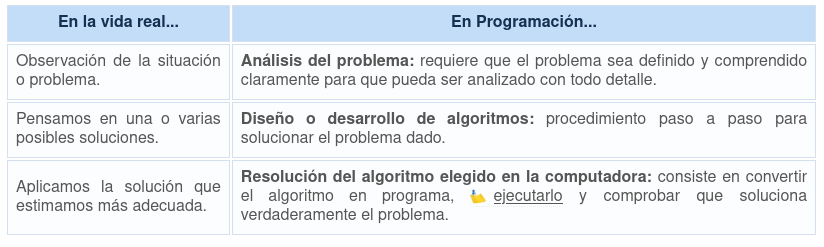
\includegraphics[scale=0.70]{pasos-problemas.png}
    \caption{Pasos para la resolución de un problema}
\end{figure}

Para que una \textbf{solución} se considere \textbf{correcta} tiene que tener principalmente dos características:

\begin{itemize}
    \item \textbf{Corrección y Eficacia}: si resuelve el problema de forma adecuada.
    \item \textbf{Eficiencia}: si lo realiza en un tiempo mínimo y con un uso óptimo de los recursos del sistema.
\end{itemize}

Para construir esta solución, hay que tener en cuenta algunos conceptos ligados a la programación, como son:

\begin{enumerate}
    \item \textbf{Abstracción}: se trata de realizar una análisis del problema para descomponerlo en problemas más pequeños y de menos complejidad de manera precisa. \textbf{Divide y Vencerás}: es una filosofía general para resolver problemas y de aquí que no solo forme parte del vocabulario informático, sino que también se utiliza en otros muchos ámbitos.

    \item \textbf{Encapsulación}: consiste en ocultar la información de un objeto o función de forma que se pueda implementar de diferentes maneras sin que esto afecte al resto de objetos.

    \item \textbf{Modularidad}: estructuraremos cada parte en módulos independientes, cada uno con su función correspondiente.
\end{enumerate}

Todo estos conceptos, deberemos tenerlos en cuenta a la hora de analizar el problema, para llegar a un solución lo más óptima posible.

\subsection{Algoritmos y Programas}
Una vez realizado el análisis del problema, tenemos que diseñar y desarrollar un \textbf{algoritmo} adecuado que pueda solucionarlo. Pero, ¿que es un algoritmo?

Un \textbf{algoritmo} es una secuencia ordenada de pasos, descrita sin ambigüedades, que conducen a la solución de un problema.

Los algoritmos deben ser \textbf{independientes} de los \textbf{lenguajes de programación} y de las \textbf{computadoras} donde se ejecutan, de forma que puedan implementarse sobre cualquier ordenador empleando cualquier lenguaje de programación. Esto facilita que una misma solución pueda emplearse para el mismo problema en diferentes dispositivos.

La \textbf{diferencia} entre un algoritmo y un \textbf{programa} es que en este último lo pasos deben escribirse en un \textbf{lenguaje de programación concreto} para que pueda ser ejecutado en el ordenador y así obtener la solución deseada.

Los \textbf{lenguajes de programación} son solo un medio para expresar el algoritmo y el ordenador un procesador para ejecutarlo. El diseño de algoritmos es una tare que requiere de la creatividad y conocimientos de las técnicas de programación del programador, así, diferentes programadores pueden desarrollar diferentes algoritmos para resolver un mismo problema.

Las principales \textbf{características} que debe cumplir un \textbf{algoritmo} son:

\begin{itemize}
    \item Debe ser \textbf{preciso} e indicar el orden en el que se realiza cada paso.
    \item Debe estar \textbf{bien definido}, si se ejecuta dos o más veces, debemos obtener el mismo resultado.
    \item Debe ser \textbf{finito}, teniendo un número de pasos bien determinado.
\end{itemize}

Cuando los problemas complejos, debemos descomponer estos en subproblemas más simples, y estos a su vez en otros más pequeños. Es lo que se conoce como \textbf{diseño descendente} o \textbf{diseño modular} y se basa en el lema \textbf{Divide y Vencerás}.

Para \textbf{representar gráficamente} los algoritmos tenemos diferentes herramientas que nos ayudarán a describir su comportamiento de una forma precisa y genérica, que nos facilitará la implementación del algoritmo en diferentes lenguajes de programación. Las principales herramientas que tenemos son:

\begin{itemize}
    \item \textbf{Diagramas de Flujo}: esta técnica utiliza símbolos gráficos para representar el flujo de ejecución del algoritmo y suelen ser empleados en la fase de análisis.
    \item \textbf{Pseudocódigo}: se basa en el uso de palabras clave en lenguaje natural, representando las constantes, variables y otras estructuras de programación de forma escrita. Es la técnica mas utilizada actualmente.
    \item \textbf{Tablas de Decisión}: es un tabla que representa las diferentes condiciones del problema con sus respectivas acciones. Suele ser una técnica de apoyo a pseudocódigo cuando existen circunstancias condicionales complejas.
\end{itemize}

\section{Fases de la Programación}
Sea cual sea el estilo que escojamos para resolver el problema, deberemos realizar el proceso aplicando un método a nuestro trabajo. Así, el \textbf{proceso de creación de software} se puede dividir en las siguientes \textbf{fases}:

\begin{itemize}
    \item \textbf{Fase de resolución del problema}
    \item \textbf{Fase de implementación}
    \item \textbf{Fase de explotación y mantenimiento}
\end{itemize}

En los siguientes puntos, analizaremos cada una de estas fases.

\subsection{Resolución del Problema}
Esta es la primera fase del desarrollo del programa, para la cuál deberá estar bien definido cual es el problema que se quiere solucionar y tener un comprensión clara de éste para poder realizar su análisis y diseño. Esta fase se puede dividir en \textbf{dos etapas}:

\begin{enumerate}
    \item \textbf{Etapa de Análisis}:

    En esta primera etapa se debe analizar el problema, lo que nos va a indicar las especificaciones y requisitos que la aplicación debe cumplir. Para llevar esto acabo, se deberán realizar diferentes entrevistas entre el programador y el cliente/usuario para precisar cuales son las características que debe tener la aplicación, especificando, entre otras cosas, los procesos y estructuras que deberá tener ésta. La creación de \textbf{prototipos} será muy útil en esta fase para saber con mayor exactitud los puntos a tratar.

    Esta etapa proporcionará una idea general de lo que se solicita, realizando sucesivos refinamientos posteriormente que servirá para determinar cual es la información que ofrecerá la resolución del problema y que datos son necesarios para resolver este.

    \item \textbf{Etapa de Diseño}:

    En esta tapa se convierte la especificación de la etapa de análisis en un diseño más detallado que define el comportamiento o la secuencia lógica de instrucciones capaz de resolver el problema planteado. Estos pasos sucesivos, constituyen lo que ya hemos definido como algoritmo.

    Antes de pasar a la implementación del algoritmo, tenemos que tener claro que la solución que se propone es la adecuada. Para ello, toda solución necesitará de la \textbf{prueba} o \textbf{traza} del programa. Este procedimiento consistirá en el seguimiento paso a paso de cada instrucción del algoritmo utilizando los datos correctos. Si la solución aportada contiene errores, deberemos volver a la etapa de análisis, si no, podremos pasar a la fase de implementación.
\end{enumerate}

\subsection{Implementación}
Esta fase consiste en plasmar en un código la solución a la que hemos llegado en la fase de resolución del problema y consta de las siguientes etapas:

\begin{enumerate}
    \item \textbf{Etapa de Codificación}:

    Esta etapa consiste en transformar o traducir la solución a la que hemos llegado en un lenguaje de programación concreto. Para comprobar la estabilidad y calidad de la solución, deberemos realizar una serie de pruebas para comprobar que los módulos funcionan correctamente (\textbf{pruebas unitarias}), que dichos módulos funcionan bien entre ellos (\textbf{pruebas de interconexión}) y todo el conjunto funciona correctamente (\textbf{pruebas de integración}).

    Cuando realizamos la traducción deberemos tener en cuenta la reglas gramaticales y sintácticas del lenguaje de programación que estemos usando, lo que generará lo que se conoce como \textbf{código fuente}, es decir, el programa en sí mismo. Pero para que nuestro programa funcione correctamente, antes deberá ser traducido a \textbf{código máquina}, el único lenguaje que entiende el ordenador. Este proceso de traducción será llevado a cabo por un \textbf{compilador} o un \textbf{interprete}, dependiendo del lenguaje de programación que estemos empleando.

    Algunos de los términos que están asociados a esta fase son los siguientes:

    \begin{itemize}
        \item \textbf{Compilación}: proceso mediante el cual el código fuente, es decir, el conjunto de instrucciones escritas en un determinado lenguaje de programación, es traducido a código máquina, un código binario que es el único lenguaje que entiende el computador.

        \item \textbf{Compilador}: es la aplicación informática que se encarga de realizar la traducción. Esta recibe el código fuente, y tras realizar una análisis lexicográfico, semántico y sintáctico, generando en primer lugar un código intermedio sin optimizar, el cual se optimiza y genera el código objeto para la plataforma especifica.

        \item \textbf{Interprete}: aplicación informática capaz de analizar y traducir programas escritos en un determinado lenguaje de programación. A diferencia de los compiladores, que realizan una traducción completa del programa a lenguaje máquina, los interpretas van realizando la traducción a medida que va siendo necesaria, típicamente, realizándola instrucción por instrucción. Además, no suelen guardar los resultados de dicha traducción.
    \end{itemize}

    \item \textbf{Prueba, Ejecución y Validación}:

    Una vez que el programa ha sido codificado, estará listo para ser ejecutado. Para ello, deberemos implantar la aplicación en el sistema donde va a ser ejecutado para comprobar su funcionamiento correcto. Utilizando diferentes datos, se comprobará si el programa cumple con los requisitos que se han especificado, si se detectan nuevos errores o si la interfaz es amigable. Se trata de poner a prueba nuestro programa para ver su respuesta en diferentes situaciones.

    Mientas que el programa tenga errores, no podremos pasar a la siguiente fase. Una vez que se corrijan, se habrán generado diferentes documentos sobre la aplicación que entrarán el alguna de las siguientes dos categorías:

    \begin{itemize}
        \item \textbf{Documentación Interna}: encabezados, descripciones, declaraciones del problema y comentarios que se incluyen dentro de código fuente.

        \item \textbf{Documentación Externa}: son los manuales que se crean para una mejor ejecución y utilización del programa, así como los diferentes diagramas generados durante el proceso de desarrollo que nos ayuden a comprender mejor su funcionamiento y arquitectura.
    \end{itemize}
\end{enumerate}

\subsection{Explotación}
En esta última fase, el software ya esta instalado en el sistema y esta siendo de utilidad para los usuarios, siendo esta la \textbf{etapa de explotación}.

Periódicamente será necesario realizar evaluaciones y, si es necesario, llevar a cabo modificaciones para que el programa se adapte o actualice a las nuevas necesidades de los usuarios, pudiendo también realizarse la corrección de errores no detectados anteriormente. Esta es la \textbf{etapa de mantenimiento}.

Así, se define el \textbf{mantenimiento de software} como el proceso de mejora y optimización del software después de su entrega al usuario final. Involucra la realización de cambios para corregir defectos y dependencias encontradas durante su uso o para la adición de funcionalidades para mejorar su usabilidad y aplicabilidad.

Sera indispensable que se haya generado la documentación adecuada para facilitar la labor del programador en la compresión, uso y modificación de la aplicación.

\section{Ciclo de Vida del Software}
Sean cuales sean las fases que las fases en las que realicemos el proceso de desarrollo de software, siempre habrá que aplicar un \textbf{modelo de ciclo vida}, siendo este una sucesión de estados o fases por las cuales pasa el software a lo largo de su vida.

Este proceso debe tener siempre la siguientes etapas mínimas:

\begin{itemize}
    \item \textbf{Especificación} y \textbf{Análisis de Requisitos}
    \item \textbf{Diseño}
    \item \textbf{Codificación}
    \item \textbf{Pruebas}
    \item \textbf{Instalación} y \textbf{Producción}
    \item \textbf{Mantenimiento}
\end{itemize}

Existen diferentes modelos de desarrollo como el modelo en cascada, en espiral, incremental, evolutivo, etc.. En la siguiente \href{https://es.wikipedia.org/wiki/Proceso_del_desarrollo_del_software}{entrada de Wikipedia} podemos ver más información sobre el proceso de desarrollo de software y las diferentes metodologías.

\section{Lenguajes de Programación}
Como hemos visto en los puntos anteriores, una de las etapas del desarrollo es la codificación del programa. Para ello, emplearemos un lenguaje que exprese cada uno de los pasos que se deben ejecutar. Este lenguaje recibe el nombre de \textbf{lenguaje de programación}.

Se entiende por \textbf{lenguaje de programación} el conjunto de reglas sintácticas y semánticas, símbolos y palabras especiales establecidos para la construcción del programa. Todo lenguaje se compone de:

\begin{itemize}
    \item \textbf{Gramática}: reglas aplicables al conjunto de símbolos y palabras empleados en el lenguaje de programación para la construcción de sentencias correctas.
    \item \textbf{Léxico}: es el conjunto de símbolos y palabras especiales, es decir, el vocabulario del lenguaje.
    \item \textbf{Sintaxis}: son las posibles combinaciones de símbolos y palabras especiales.
    \item \textbf{Semántica}: es el significado de cada construcción del lenguaje, es decir, la acción que se llevará a cabo.
\end{itemize}

Los lenguajes permiten que los programadores pueden expresar el código de forma que sea legible para ellos y otros programadores. Estos se clasifican según lo cercanos que estén al lenguaje máquina o al lenguaje natural, así como si son lenguajes interpretados o compilados, lo que vamos a ver en los siguientes puntos.

\subsection{Lenguaje Máquina}
Este lenguajes es él único que entiende el ordenador y se compone de un conjunto de instrucciones codificadas en binario que se encarga de ejecutar el procesador. Este lenguaje es directamente interpretable por un circuito microprogramable.

Se trata del primer lenguaje utilizado para la programación de computadoras. De hecho, cada máquina tenía su propio conjunto de instrucciones codificadas en ceros y uno. Esto, evidentemente, genera un conjunto de \textbf{inconvenientes}:

\begin{itemize}
    \item Cada programa era válido \textbf{solo para un tipo de procesador} u ordenador.
    \item La \textbf{lectura} e \textbf{interpretación} de este tipo de programas es \textbf{extremadamente difícil}, por lo que realizar modificaciones resultaba extremadamente costoso.
    \item Los programadores de la época debían \textbf{memorizar largas cadenas de unos y ceros}, que equivalían a las instrucciones disponibles en los diferentes tipos de procesadores.
    \item Además, la introducción de estas cadenas suponía \textbf{largos tiempos de espera y posibles errores}.
\end{itemize}

En la siguiente tabla muestran algunos ejemplos de operaciones codificadas en binario.

\begin{figure}[H]
    \centering
    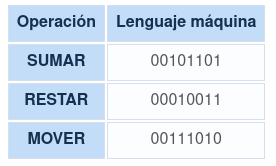
\includegraphics[scale=1]{ejemplo-binario.png}
    \caption{Operaciones en binario}
\end{figure}

Dada la dificultad de este lenguaje, con el tiempo fue sustituido por otros de más fácil compresión, aunque hay que tener en cuenta que en última instancia todos los lenguajes deben ser traducido a éste para que puedan ser interpretados y ejecutados por el ordenador.

\subsection{Lenguaje Ensamblador}
La evolución del lenguaje máquina fue el \textbf{lenguaje ensamblador}. En éste, las instrucciones ya no son secuencias binarias sino que son códigos de operación que describen operaciones básicas del procesador.

Estos códigos, conocidos como \textbf{mnemotécnicos}, son palabras especiales que sustituyen largas secuencias de unos y ceros, utilizadas para referirse a diferentes operaciones disponibles en el juego de instrucciones que soporta un procesador concreto.

En la siguiente tabla, podemos ver alguno ejemplos de estos mnemotécnicos con diferentes operaciones.

\begin{figure}[H]
    \centering
    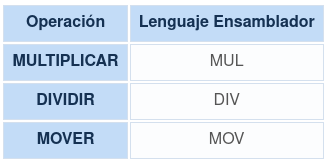
\includegraphics[scale=1]{ejemplo-asm.png}
    \caption{Operaciones en ensamblador}
\end{figure}

Aunque el ensamblador fue un intento de acercar el lenguaje máquina al lenguaje humano, aún presentaba diferentes \textbf{dificultades}:
\begin{itemize}
    \item Los programas seguían \textbf{dependiendo} directamente del \textbf{hardware} que los soportaba.
    \item Los programadores debían \textbf{conocer} detalladamente \textbf{la máquina} sobre la que programaban, ya que debían hacer un uso adecuado de los recursos del sistema.
    \item La \textbf{lectura}, \textbf{interpretación} o \textbf{modificación} de los programas seguía presentando dificultades.
\end{itemize}

Todo programa escrito en ensamblador necesita ser traducido al lenguaje máquina para poder ser ejecutad. Esta función la lleva a cabo el \textbf{programa ensamblador}, el cual convierte el programa original escrito en lenguaje ensamblador (código fuente) en el programa traducido a lenguaje máquina (código objeto).

\subsection{Lenguajes Compilados}
Para paliar los defectos del lenguaje ensamblador y acercar los lenguajes de programación al lenguaje humano nacieron los \textbf{lenguajes compilados}.

 Así surgieron lenguajes como \textbf{Pascal}, \textbf{FORTRAN}, \textbf{Algol}, \textbf{C}, \textbf{C++}, etc. Estos lenguajes, más cercanos al humano, también se denominan \textbf{lenguajes de alto nivel}. Son más fáciles de utilizar y comprender, ya que las instrucciones que emplean y los signos que usan son fácilmente reconocibles por el programador.

 Entre las principales \textbf{ventajas} de estos lenguajes tenemos:
 \begin{itemize}
     \item Son mucho más \textbf{fáciles} de \textbf{aprender y utilizar} que sus predecesores.
     \item Se \textbf{reduce} el \textbf{tiempo} para desarrollar programas así como el \textbf{coste}.
     \item Son \textbf{independientes del hardware}, es decir, los programas pueden ejecutarse en diferentes tipos de máquina.
     \item La \textbf{lectura}, \textbf{modificación} e \textbf{interpretación} de los programas es \textbf{mucho más sencilla}.
 \end{itemize}

Un programa que este escrito en un lenguaje de alto nivel también tiene que \textbf{traducirse} a código máquina para que pueda ser ejecutado por el ordenador. Este trabajo, lo lleva a cabo el \textbf{compilador}, mediante un proceso de traducción que se conoce como \textbf{compilación}.

En la siguiente imagen podemos ver de forma mas ilustrativa cual es el proceso de compilación.

\begin{figure}[H]
    \centering
    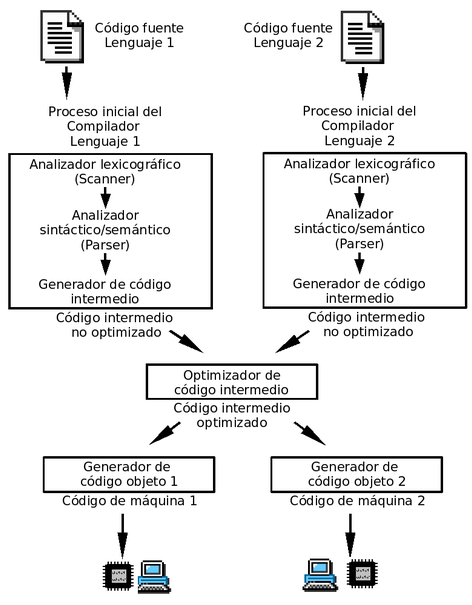
\includegraphics[scale=0.50]{compilador.png}
    \caption{Proceso de compilación}
\end{figure}

El compilador realizará la traducción y ademas \textbf{informará} de posibles \textbf{errores}. Una vez subsanados se generará el programa traducido a código máquina, conocido como \textbf{código objeto}. Este programa aún no puede ser ejecutado hasta que no se añadan los módulos de enlace o bibliotecas, durante el proceso de enlazado. Una vez realizado, se obtiene el \textbf{código ejecutable}.

\subsection{Lenguaje Interpretados}
Los lenguajes interpretados están diseñados para que su ejecución se realice a través de un \textbf{interprete}. Cada instrucción de un lenguaje interpretado se analiza, traduce y ejecuta tras haber sido verificada.

Un \textbf{interprete} es un traductor de lenguaje de alto nivel donde el proceso de traducción y ejecución se llevan a cabo simultáneamente, es decir, la instrucción se pasa al lenguaje máquina y se ejecuta directamente. No se genera código objeto ni ejecutable, como en los lenguajes compilados.

Los lenguajes interpretados tienen el inconveniente que son un poco más lentos que los lenguajes compilados, además, se necesita tener el intérprete instalado en la máquina donde se quiere ejecutar el programa, algo que no es necesario con los lenguajes compilados.

Algunos ejemplos de lenguajes interpretados son \textbf{Perl}, \textbf{PHP}, \textbf{Python} o \textbf{Javascript}, entre otros.

A medio camino entre los lenguajes compilados y los interpretados existen los lenguajes que podríamos llamar \textbf{pseudo-compilados} o \textbf{pseudo-interpretados}, como es el caso de \textbf{Java}. Java puede verse como un lenguaje compilado, pero también como un lenguaje interpretado, ya que su código fuente se compila para obtener el código binario conocido como \textbf{bytecode}, que son estructuras parecidas a las instrucciones máquina, con la importante propiedad de no se dependiente de ningún tipo de máquina. La \textbf{Maquina Virtual Java} se encargará de interpretar este código, y para su ejecución, lo traducirá al código máquina del procesador en particular donde se quiera ejecutar la aplicación.

\section{El Lenguaje de Programación Java}
Java es un lenguaje de programación con un sintaxis similar a C++, donde se han eliminado algunos de sus elementos complicados, como el tratamiento de punteros. Es un lenguaje \textbf{orientado a objetos} que nos permite la utilización de gran cantidad de bibliotecas fomentando la reutilización de código y evitando que tengamos que reescribir código ya existente.

Una de las principales virtudes de Java es su \textbf{independencia del hardware}, ya que el código que se genera es válido para cualquier plataforma. Este código será ejecutado en una maquina virtual denominada \textbf{Máquina Virtual Java} (JVM), que interpretará el código generado traduciéndolo al código máquina de la plataforma donde queramos ejecutarlo. De este modo, el programa se escribe una única vez y puede hacerse funcionar en cualquier lugar, llevando a la práctica el lema del lenguaje \textbf{``Write once, run everywhere''}.

Antes de la aparición de Java, el lenguaje de programación C era uno de los más versátiles y extendidos, pero cuando los programas en C aumentaban de volumen, su manejo se volvía muy complejo. Aunque mediante la programación modular y estructura se conseguía reducir esta complejidad, no era suficiente.

Fue entonces cuando entró en escena la \textbf{Programación Orientada a Objetos} (POO), aproximando más la construcción al pensamiento humano y haciendo más sencillo todo el proceso. Los problemas se dividen en objetos que tienen propiedades e interactúan con otros objetos, pudiendo el programador centrarse en cada objeto y los detalles las propiedades y funcionalidades que este posee. Fue entonces cuando surgió el lenguaje Java.

Las principales \textbf{características} del \textbf{lenguaje Java} son:

\begin{itemize}
    \item El código generado por el compilador es independiente del hardware.
    \item Es totalmente orientado a objetos.
    \item Su sintaxis es similar a C y C++.
    \item Es distribuido, es decir, preparado para aplicaciones TCP/IP.
    \item Dispone de un amplio conjunto de bibliotecas.
    \item Es robusto, realizando comprobaciones tanto en tiempo de compilación como de ejecución.
    \item La seguridad está garantizada, ya que las aplicaciones Java no acceden directamente a zonas delicadas de la memoria o el sistema.
\end{itemize}

\subsection{Breve Historia de Java}
Java surgió en 1991 cuando un pequeño grupo de ingenieros de Sun Microsystems trataron de diseñar un lenguaje de programación destinado a programar pequeños dispositivos electrónicos. El problema con estos dispositivos es que cambian rápidamente de un modelo a otro y el software debe ser reescrito, por lo que necesitaban un lenguaje que se fuera \textbf{independiente del dispositivo}.

No fue hasta 1995 cuando el lenguaje adoptó el nombre de Java, dándose a conocer al mundo como lenguaje de programación de computadores. El hecho de que sea un lenguaje orientado a objetos, independiente de la plataforma y su facilidad para la creación de aplicaciones TCP/IP, han hecho que Java sea uno de los lenguajes más utilizados.

El factor determinante para su expansión fue la inclusión de un interprete en la versión 2.0 del navegador Netscape, lo que supuso un gran revuelo en internet. A principio de 1997 apareció \textbf{Java 1.1}, que proporcionó sustanciales mejoras en el lenguaje. A finales de 1998 salió \textbf{Java 1.2}, posteriormente rebautizado como \textbf{Java 2}.

Para el desarrollo de programas en Java es necesario el uso de un entorno de desarrollo denominado \textbf{JDK} (Java Development Kit), que provee de un compilador y un entorno de ejecución, conocido como \textbf{JRE} (Java Runtime Environment), para ejecutar los bytecode generados. Al igual que el lenguaje, JDK y JRE han sido mejorados con cada versión del lenguaje.

\textbf{Java 2} es la tercera versión del lenguaje, pero no solo incluye el lenguaje, sino incluye:

\begin{itemize}
    \item El lenguaje de programación: Java.
    \item Un conjunto de bibliotecas estándar que vienen incluidas en el lenguaje y son necesarias en todo el entorno Java. Es el \textbf{Java Core}.
    \item Un conjunto de herramientas para el desarrollo de programas como compilador de bytecode, el generador de documentación, un depurador, etc...
    \item Un entorno de ejecución que en definitiva es una máquina virtual para ejecutar los bytecodes generados.
\end{itemize}

En la siguiente imagen podemos ver un esquema de los elementos de Java 2.

\begin{figure}[H]
    \centering
    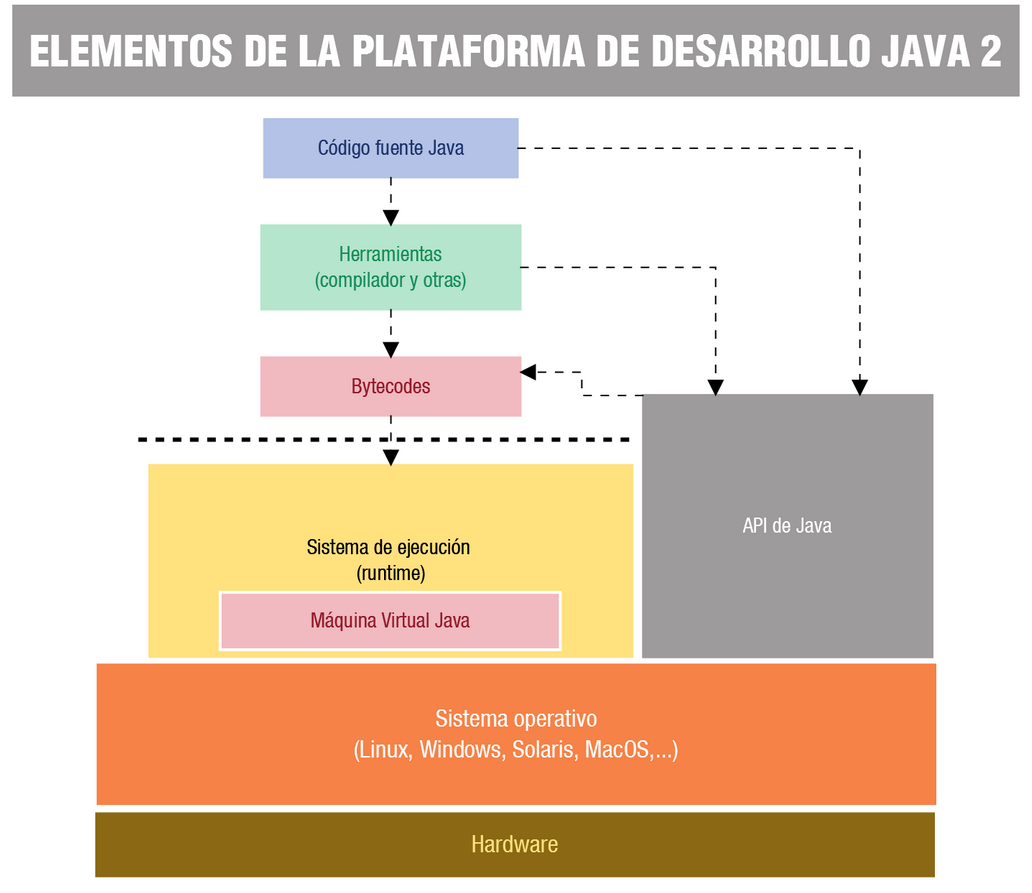
\includegraphics[scale=0.35]{java2.png}
    \caption{Elementos de Java 2}
\end{figure}

Actualmente hay varias ediciones de la plataforma Java y que de forma resumida se podrían clasificar en:

\begin{itemize}
    \item \textbf{Java SE}: es la plataforma base para el desarrollo de aplicaciones con Java. Es usado para desarrollar aplicaciones de escritorio, applets y otros tipos de aplicaciones. Es fundamental, ya que es la basa en la que se cimienta el resto de plataformas Java.
    \item \textbf{Java EE}: es una plataforma de desarrollo de aplicaciones empresariales y del lado del servidor.
    \item \textbf{Java ME}: es una plataforma de desarrollo de aplicaciones para dispositivos móviles.
\end{itemize}

En \href{https://www.campusmvp.es/recursos/post/Descifrando-Java-lenguaje-plataforma-ediciones-implementaciones.aspx}{este enlace} puedes encontrar más información sobre las diferentes plataformas de Java y como trabajan entre ellas.

\subsection{La POO y Java}
En Java, los datos y el código (funciones o métodos) se combinan en entidades llamadas \textbf{objetos}. El objeto tendrá un \textbf{comportamiento} (su código interno) y un \textbf{estado} (los datos). Los objetos permiten la reutilización de código y pueden considerarse a sí mismos con piezas reutilizables en diferentes proyectos. Esta característica permite reducir el tiempo de desarrollo de aplicaciones.

Al incorporar los conceptos de Programación Orientada a Objetos (POO), Java incluye las tres características propias de este paradigma de programación:

\begin{itemize}
    \item \textbf{Encapsulación}: se denomina así al ocultamiento de la información interna de un objeto. Este solo se puede modificar a través de sus operaciones definidas.
    \item \textbf{Herencia}: mecanismo que permite derivar una clase de otra, de manera que extienda su funcionalidad.
    \item \textbf{Polimorfismo}: capacidad para que varias clases derivada de otra utilicen un mismo método de forma diferentes.
\end{itemize}

Los patrones o tipos de objetos se denominan \textbf{clases} y los objetos que utilizan estos patrones o pertenecen a dichos tipos se denominan \textbf{instancias}.

En la siguiente figura podemos ver algunas de las ventajas de la POO de forma más esquemática.

\begin{figure}[H]
    \centering
    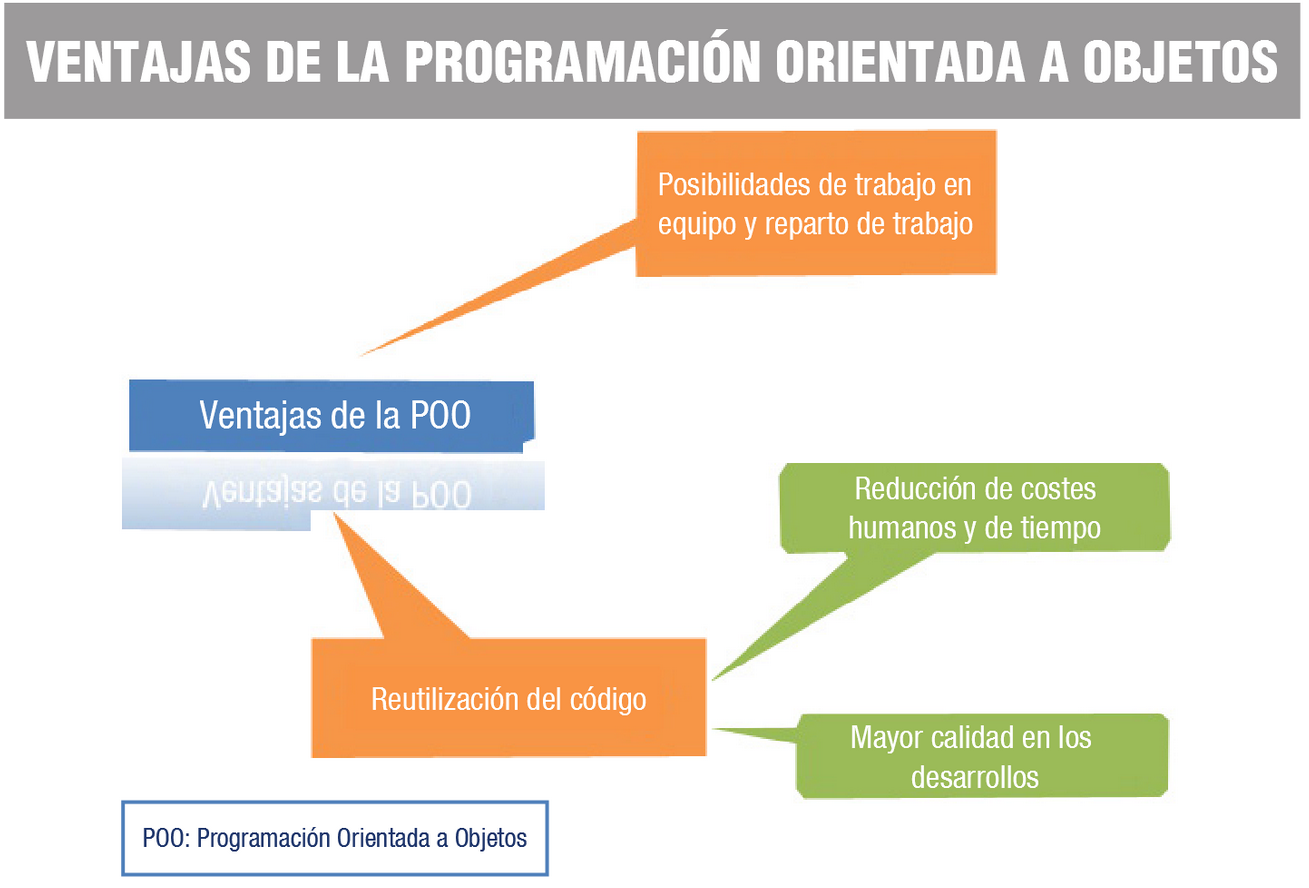
\includegraphics[scale=0.30]{ventajas-poo.png}
    \caption{Ventajas de la POO}
\end{figure}

\subsection{Independencia de la Plataforma}
Hay dos características de distinguen a Java de otros lenguajes de programación, como son la \textbf{independencia de la plataforma} y la posibilidad de \textbf{crear aplicaciones} para \textbf{trabajar en red}.

Estas características consisten en:
\begin{itemize}
    \item \textbf{Independencia}: los programas escritos en Java pueden ser ejecutados en cualquier tipo de hardware. El código fuente se compila generando el código conocido como Java Bytecode, el cual será interpretado y ejecutado por la \textbf{Máquina Virtual Java}, que es un programa escrito en código nativo de la plataforma destino. Con eso se evita tener que realizar un programada diferente para diferentes CPUs.

    \item \textbf{Trabajo en red}: esta capacidad del lenguaje ofrece múltiples posibilidades para la comunicación vía TCP/IP. Para poder hacer esto, existen librerías que permiten el acceso y la interacción con protocolos como \textbf{http}, \textbf{ftp}, etc.., facilitando las tareas del programador para el tratamiento de la información.
\end{itemize}

\subsection{Seguridad y Simplicidad}
Además de las características vistas en el punto anterior, cabe destacar dos virtudes de este lenguaje que hacen que este tan extendido: la \textbf{seguridad} y la \textbf{simplicidad}.

\begin{itemize}
    \item \textbf{Seguridad}: en primer lugar, el acceso a zonas sensibles de memoria que podemos tener en otros lenguajes como C o C++ se han eliminado en Java.

    En segundo lugar, el código en Java se comprueba y verifica para evitar que determinadas secciones del código produzcan efectos adversos. Los test que se aplican garantizan que las operaciones, operandos, conversiones y uso de clases son seguras.

    En definitiva, podemos afirmar que Java es un lenguaje seguro.

    \item \textbf{Simplicidad}: aunque Java es tan potente como C o C++, es bastante más sencillo. Tiene una curva de aprendizaje muy rápida y para alguien que aprende a programar con este lenguaje, le resultará más fácil comenzar a escribir aplicaciones interesantes.

    Java elimina ciertos mecanismos complejos que si encontramos en C o C++ como pueden ser la aritmética de punteros, los registros, la definición de tipos, la gestión de memoria, etc.., reduciendo considerablemente la posibilidad de cometer errores comunes en otros lenguajes de programación.

    Un elemento que ayuda a la simplicidad de Java es el \textbf{Recolector de Basura} (Garbage Collector), que permite al programador liberarse de la gestión de memoria y hace que ciertos bloques de memoria puedan reaprovecharse, disminuyendo el número de huevos libres, lo que se conoce como \textbf{fragmentación de memoria}.
\end{itemize}

Como vemos, además de ser independiente de la plataforma, Java es un lenguaje más seguro y simple que otros parecidos, manteniendo la misma potencia que estos.

\subsection{Java y los Bytecodes}
Un programa en Java no es directamente ejecutable, es necesario que el código sea interpretado por la Máquina Virtual.

Una vez escrito el código fuente (con extensión .java), este es precompilado generándose los códigos de bytes o Bytecodes (con extensión .class), que serán interpretados directamente por la Máquina Virtual y traducidos a código nativo de la plataforma donde queramos ejecutarlo.

Un \textbf{Bytecode} es un conjunto de instrucciones en lenguaje máquina que no son específicos de ningún procesador o sistema de cómputo. Un intérprete de bytes para una plataforma concreta será el que los ejecute. A este interprete también se les conoce como Máquina Virtual Java.

En el proceso de compilación, existe un verificador de códigos de bytes que se asegurará que se cumplen las siguientes condiciones:

\begin{itemize}
    \item El código satisface las especificaciones de la Máquina Virtual Java.
    \item No existe amenaza contra la integridad del sistema.
    \item No se produce desbordamiento de memoria.
    \item Los parámetros y sus tipos son adecuados.
    \item No existen conversiones de datos no permitidas.
\end{itemize}

Para que un bytecode puede ser ejecutado en cualquier plataforma es imprescindible que la plataforma cuente con el intérprete adecuado, es decir, la \textbf{máquina virtual} específica para \textbf{dicha plataforma}.

\section{Programas en Java}
Hasta ahora hemos descrito el lenguaje de programación Java y hablado un poco sobre su historia y características. En este punto, ya vamos a empezar ha hablar de los programas en Java, cuales son su elementos básicos, como debemos escribir el código y los tipos de aplicaciones que podremos crear con este lenguaje.

\subsection{Estructura de un Programa}
En la siguiente figura, se presenta una estructura general de un programa en Java, la cual vamos a explicar en esta sección punto por punto.

\begin{figure}[H]
    \centering
    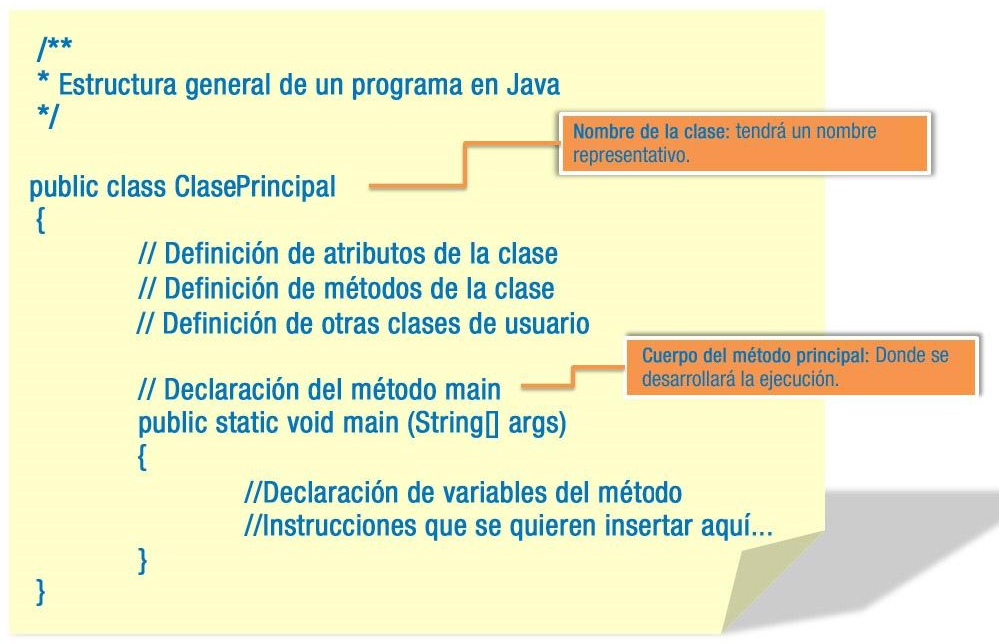
\includegraphics[scale=0.40]{estructura-java.png}
    \caption{Estructura general de un programa en Java}
\end{figure}

Los diferentes elementos que podemos ver en esta figura son los siguientes:

\begin{itemize}
    \item \textbf{public class ClasePrincipal}: todos los programas en Java deben incluir este elemento. Podrá llamarse ClasePrincipal, ProgramaPrincipal, ... o como queramos, pero debe tener un nombre. Se trata de una clase general donde se incluyen todos los demás elementos del programa. En unidades posteriores veremos que es una clase y cuales son sus componentes principales. Por ahora es suficiente que sepamos que nuestro programa debe comenzar con este elemento.

    \item \textbf{public static void main (String args[])}: dentro del elemento anterior podemos ver el método \textbf{main()} que contiene las líneas de código de nuestro programa. Más adelante también veremos que es un método. Basta saber por ahora que al igual que la línea anterior nuestro programa debe contener la sentencia \textbf{public static void main (String args[])}. Aquí dentro podremos incluir las instrucciones que veamos oportunas para ejecución del programa.

    \item \textbf{Comentarios}: los comentarios suelen introducirse en el programa para realizar aclaraciones, anotaciones o cualquier otra indicación que el programador estime oportuna. Estos comentarios pueden introducirse de dos formas:

    \begin{itemize}
        \item Con \textit{\textbf{//}} estaríamos estableciendo una línea de comentario, es decir, todo lo que hay detrás de este símbolo es un comentario hasta que se produzca un salto de línea.
        \item Si queremos indicar que un comentario tiene varias líneas debemos usar \textit{\textbf{/*} }para comenzar el comentario y \textit{\textbf{*/}} para cerrarlo.
    \end{itemize}

    \item \textbf{Bloques de Código} (\textbf{\{} \textbf{\}}): con conjuntos de instrucciones que se marcan mediante la apertura y cierre de llaves \textbf{\{} \textbf{\}}. En código así marcado se considera interno al bloque.

    \item \textbf{Punto y Coma} (\textbf{;}): aunque en el ejemplo de la imagen no tenemos ninguna línea de código acabada con un punto y coma, para no distraernos de momento con estos detalles, hay que hacer hincapié en que cada línea de código ha de terminar con un punto y coma. En caso de no hacerlo, tendremos errores sintácticos.
\end{itemize}

\subsection{El Entorno Básico de Desarrollo de Java}
La herramienta básica para comenzar a desarrollar aplicaciones en Java es el \textbf{JDK} (\textbf{Java Development Kit}), que incluye un compilador y un interprete para la línea de comandos. Estos dos programas son los empleados en la compilación y la interpretación del código.

Como veremos, existen diferentes entornos para el desarrollo de aplicaciones en Java que incluyen una gran variedad de herramientas, pero por ahora nos centraremos en el entorno básico, extendido y gratuito, el Java Development Kit. JDK es un entorno para construir aplicaciones, applets y componentes utilizando el lenguaje de programación Java, incluyendo todas las herramientas necesarias para su construcción y ejecución.

Junto con JDK se incluye una implementación del entorno de ejecución Java, conocido como \textbf{Java Runtime Environment} (\textbf{JRE}), para ser utilizado por JDK. El JRE incluye la \textbf{Java Virtual Machine} (\textbf{JVM}), bibliotecas de clases y otros ficheros que soportan la ejecución de programas escritos en Java.

Java fue creado por Sun Microsystems, pero posteriormente fue absorbida por Oracle, los que no han dejado de lanzar versiones de JDK. Con el lanzamiento de Java 11, Oracle hizo un cambio de licencia de modo que se convirtió en tecnología de pago en caso de usarlo en ciertas circunstancias. Podemos usar JDK u otras implementaciones abiertas. En nuestro caso, usaremos \textbf{OpenJDK}.

\textbf{OpenJDK} es la versión libre de la plataforma de desarrollo Java, en concreto de su versión \textbf{Java SE} (Standard Edition). Esta bajo la licencia \textbf{GPL 2.0} y desde la versión 7 de Java SE, OpenJDK es la versión de referencia. \cite{wiki01}

En \href{https://www.muylinux.com/2021/03/23/adoptium-working-group-adoptopenjdk-eclipse-foundation-openjdk/}{este enlace} podemos ver una guía de como instalar OpenJDK en las principales distribuciones.

\subsection{La API de Java}
Dentro del kit de desarrollo de Java que acabos de ver se incluyen gratuitamente todas las bibliotecas de Java, los que se conoce como la \textbf{API} (Advanced Programing Interface) de Java, lo que se conoce como \textbf{Biblioteca de Clases Java}. Este conjunto de bibliotecas proporcionar al programador paquetes de clases útiles para la realización de diferentes tareas dentro de un programa. Las bibliotecas están organizadas en paquetes donde cada paquete tiene un conjunto de clases relacionadas semánticamente.

En décadas pasadas una biblioteca era un conjunto de programas que contenía cientos de rutinas. Estas rutinas manejaban las tareas de todos o casi todos los programas que necesitaban. El programador podía recurrir a estar bibliotecas para para desarrollar programas con rapidez.

Una biblioteca de clases es un conjunto de clases en programación orientada a objetos. Estas clases contienen métodos que son útiles para los programadores realizando diferentes tareas. En el caso de Java, cuando descargamos el JDK obtenemos la biblioteca de clases API. Utilizar las clases y métodos de la API de Java acelera el proceso de desarrollo de los programas. También, existen diferentes bibliotecas de clases desarrolladas por terceros que contienen componentes reutilizables de software y están disponibles a través de la web.

En la \href{https://docs.oracle.com/en/java/javase/index.html}{página oficial de Oracle} podemos encontrar información más detallada sobre la API de Java.

\subsection{Afinando la Configuración}
Para que podamos compilar y ejecutar ficheros Java es necesario que realicemos unos pequeños ajustes en la configuración del sistema. Vamos a indicarle donde puede encontrar los ficheros necesarios para realizar la labores de compilación y ejecución, es esta caso los ficheros \textbf{javac.exe} y \textbf{java.exe}, así como las librerías incluidas en la API de Java y las clases de usuario. Esto lo haremos definiendo o editando las siguientes variables del sistema.

\begin{itemize}
    \item \textbf{Variable PATH}: como aún no disponemos de un IDE (Integrated Development Environment), la única forma de ejecutar programas es a través de la línea de comandos. Pero sólo podremos ejecutar programas directamente si la ruta hacia ellos esta indicada en la variable de sistema PATH. Es necesario que incluyamos la ruta hacia estos programas en nuestra variable PATH, incluyendo la ruta donde se instaló JDK hasta su directorio \textbf{bin}.

    \item \textbf{Variable CLASSPATH}: esta variable de entorno establece donde encontrar la librerías y clases de la API de Java, así como las clases creadas por el usuario. Es decir, los ficheros \textbf{.class} que se obtienen una vez compilado el código fuente de un programa escrito en Java. Es posible que en dicha ruta existan ficheros comprimidos en los formatos \textbf{zip} o \textbf{jar} que pueden ser utilizados directamente por JDK, conteniendo en su interior los archivos \textbf{class}.
\end{itemize}

\subsection{Codificación, Compilación y Ejecución de Aplicaciones}
Una vez que la configuración del entorno de Java y tenemos el código fuente de nuestro programa escrito en un archivo con extensión \textbf{.java}, la compilación de aplicaciones se realiza mediante el programa \textbf{javac} incluido en JDK.

Para llevar a cabo esta compilación deberemos usar el comando \textbf{\textit{javac archivo.java}}, desde la línea de comandos, donde archivo.java es el archivo con nuestro código fuente.

El resultado de la compilación sera un nuevo archivo con el mismo nombre que el nuestro pero con una extensión \textbf{.class}. Este es el archivo con el código a bytecode, es decir, con el código precompilado. Si en el código fuente de nuestro programa figuraran más de una clase, veremos como al realizar la compilación se generarán tantos archivos .class como clases tengamos. Además, si esta clases tenía el método \textbf{main()} podremos ejecutarlas por separado para ver el funcionamiento de dichas clases.

Para que el programa pueda ser ejecutado, siempre y cuando este incluido en el interior el método \textbf{main()}, podemos usar el interprete incluido en JDK. Para ello, usaremos el comando \textbf{\textit{java archivo}}.

Donde \textbf{java} es el interprete y \textbf{archivo} es el archivo con el código precompilado a bytecode, es decir, el archivo con extensión \textbf{.class}. Hay que destacar que no hay que incluir la extensión del archivo .class al llamar al interprete, solo debemos poner el nombre del archivo.

\subsubsection{Estandarización del Código}
Cada vez que escribamos código es importante que sigamos unas normas o estándares que nos ayuden a realizar este proceso siempre de la misma manera. De este modo todos los programas tendrán una estructura similar y nos resultará mucho más sencillo localizar los componentes en cada uno.

En caso del lenguaje Java ya hemos visto la estructura básica de un programa. A partir de aquí, vamos a desarrollar una plantilla que nos ayudará a desarrollar nuestro programas sin tener que reescribir las partes comunes una y otra vez.

Nuestra plantilla podría tener la siguiente \textbf{estructura}:

\begin{enumerate}
    \item \textbf{Declaración de la clase principal}: aquí podríamos poner el \textbf{nombre de nuestro programa}. Es decir, en lugar de llamar a la clase \textbf{ClasePrincipal}, podríamos llamar \textbf{Concurso}, \textbf{Juego}, \textbf{CalculoDeAreas}, etc. Esto es, algún nombre que nos de una pista sobre el funcionamiento de nuestro programa.

    \item \textbf{Método main}: dentro del componente anterior y encerrado entre llaves. Este nombre no se puede cambiar. En su interior estarán las líneas de código de nuestro programa:

    \begin{enumerate}
        \item \textbf{Declaración de constantes y variables}:
        \begin{enumerate}
            \item Declaración de \textbf{constantes}
            \item Declaración de \textbf{variables de entrada}
            \item Declaración de \textbf{variables de salida}
            \item Declaración de \textbf{variables auxiliares}
        \end{enumerate}
        \item \textbf{Cuerpo del Programa}
        \begin{enumerate}
            \item \textbf{Entrada de datos}
            \item \textbf{Procedimientos}
            \item \textbf{Salida de datos}
        \end{enumerate}
    \end{enumerate}
\end{enumerate}

Si seguimos esta estructura, será muy fácil analizar nuestro programas pues estarán divididos en distintos elementos con significado propio cada uno de ellos. Ahora bien, tampoco hay que ser excesivamente rígidos. Dependiendo de la naturaleza y al complejidad del	programa es posible que alguna vez estas tres partes se fundan en una, especialmente cuando el programa sea interactivo y se sigan introduciendo datos a la vez que se van procesando e incluso devolviendo resultados.

\subsubsection{Problemas con Caracteres Acentuados}
A veces cuando intentamos ejecutar un programa Java y este tiene caracteres acentuados podemos obtener símbolos extraños, en vez de dichos caracteres, especialmente si estamos trabajando con la consola de comandos.

Una solución simple que suele funcionar en la mayoría de los casos es compilar el archivo de código fuente con normalidad, indicando cuando se vaya a realizar su ejecución la opción \textit{\textbf{-Dfile.encoding}} con la codificación que queremos emplear, es decir:


\begin{tcolorbox}[sharp corners, colback=yellow!30, colframe=white!20]
    \scriptsize
    \begin{verbatim}


java -Dfile.encoding=cp850 PROG_programa1
    \end{verbatim}
\end{tcolorbox}

En este ejemplo, la página de códigos que usamos es la 850, pero se puede forzar al interprete a usar cualquier codificación que queramos, siempre y cuando este la soporte. Para saber que codificación usa nuestro sistema, podemos usar el comando \textbf{\textit{chcp}} desde la consola, que nos mostrará dicha codificación.

\subsection{Tipos de Aplicaciones en Java}
La versatilidad del lenguaje de programación Java permite al programador crear distintos tipos de aplicaciones, los cuales listamos a continuación:

\begin{itemize}
    \item \textbf{Aplicaciones de Consola}
    \begin{itemize}
        \item Son programas independientes al igual que los creados con otros lenguajes tradicionales.
        \item Se componen como mínimo de un archivo \textbf{.class} que debe contener necesariamente el método \textbf{main()}.
        \item No necesitan un navegador y se ejecutan cuando invocamos el comando \textbf{java}. Si no se encuentra el método \textbf{main()} la aplicación no podrá ejecutarse.
        \item Estas aplicaciones leen y escriben hacia y desde la entrada y salida estándar, sin ninguna interfaz de usuario.
    \end{itemize}

    \item \textbf{Aplicaciones Gráficas}
    \begin{itemize}
        \item Aquellas que utilizan clases con capacidades gráficas, como \textbf{Swing}, que es la biblioteca para la interfaz gráfica de la API de Java.
        \item Incluyen instrucciones de tipo \textbf{import}, que indican al compilador de Java que clases del paquete \textbf{javax.swing} se incluyan en la compilación.
    \end{itemize}

    \item \textbf{Applets}
    \begin{itemize}
        \item Son programas incrustados en otras aplicaciones, normalmente páginas web que se muestran en el navegador. Cuando el navegador carga una web que contienen applets, estos se descargan en el navegador y comienza su ejecución. Esto nos permite crear programas que cualquier usuario con un navegador web puede utilizar.
        \item Los applets se descargan junto con una página HTML y se ejecutan en la máquina del cliente.
        \item No tienen acceso a partes sensibles a menos que uno le de los permisos oportunos.
        \item No tienen un método principal.
        \item Son multiplataforma y pueden ejecutarse en cualquier navegador que soporte Java.
    \end{itemize}

    \textbf{Servlets}
    \begin{itemize}
        \item Son componente de la parte del servidor de Java EE, encargados de generar respuestas a las peticiones realizadas por los usuarios.
        \item Al contrario que los applets, están pensados para trabajar en el lado del servidor y procesar las peticiones de los clientes.
    \end{itemize}

    \item \textbf{Midlets}
    \begin{itemize}
        \item Son aplicaciones Java creadas para su ejecución en sistemas de propósito simple o móviles.
        \item Se usan en dispositivos embebidos, mas específicamente para la máquina virtual Java Micron Editio (Java ME).
        \item Generalmente son juegos y aplicaciones que se ejecutan en teléfonos móviles.
    \end{itemize}
\end{itemize}

Como vemos, la variedad de aplicaciones que podemos crear con Java es enorme, ya dependerá de lo que estemos interesados en crear, usaremos unas u otras opciones y librerías.

\section{Entornos Integrados de Desarrollo}
En los comienzos de Java la utilización de la línea de comandos era algo habitual. El programador escribía el código utilizando un editor de textos básico y a continuación utilizaba el compilador para obtener el código compilado. En un paso posterior necesitaba usar una herramienta para ensamblar el programa. Por último, podía probar el programa desde la línea de comandos. El problema surgía cuando ocurría algún error y había que iniciar el proceso de nuevo.

Esto hacía que el proceso de desarrollo no estuviera optimizado. Con el paso del tiempo se fueron desarrollando aplicaciones que incluían todas las herramientas necesarias para que el proceso de desarrollo fuera más rápido, sencillo y fiable. Para cada lenguaje de programación existen múltiples entornos de desarrollo, cada uno con sus ventajas e inconvenientes. Dependiendo de las necesidades y gustos del programador, se elegirá uno u otro.

Para el lenguaje de programación Java existen diferentes alternativas, siendo los principales entornos de desarrollo \textbf{Netbeans}, desarrollado por Sun y \textbf{Eclipse}. Ambos gratuitos, con soporte de idiomas y multiplataforma (Windows, Linux y MacOS).

En nuestro caso, el entorno que vamos a usar durante nuestros desarrollos va a ser \textbf{Netbeans}, ya que es de código abierto y además ha sido desarrollado por la misma compañía que desarrollo el lenguaje Java.

\subsection{¿Que es un IDE?}
Los \textbf{IDE} (Integrated Development Environment) son aplicaciones que permiten llevar todo el proceso de desarrollo de software a través de una misma aplicación. Podremos realizar labores de edición, compilación, depuración, detección de errores, corrección y ejecución de programas escritos en Java o en otros lenguajes de programación bajo un entorno gráfico. Junto a estas características, cada entorno añade otras que ayudan a realizar el proceso de programación, como por ejemplo: resaltado de sintaxis, plantillas de diferentes tipos de aplicaciones, creación de proyectos, etc...

Hay que tener en cuenta que un IDE es solo una fachada para el proceso de desarrollo, por lo que tendremos que tener instalados compiladores, interpretes y demás para su correcto funcionamiento.

\subsection{IDE Actuales}
Existen una gran variedad de IDEs en el mercado para el lenguaje de programación Java, orientados a principiantes, para profesionales, gratuitos, de pago, libres, propietarios, etc. A continuación damos una lista de los principales.

\begin{itemize}
    \item IDEs Gratuitos y de Libre Distribución:
    \begin{itemize}
        \item \textbf{Netbeans}
        \item \textbf{Eclipse}
        \item \textbf{BlueJ}
        \item \textbf{jGRASP}
        \item \textbf{JCreator LE}
    \end{itemize}

    \item IDEs Propietarios:
    \begin{itemize}
        \item \textbf{IntelliJ IDEA}
        \item \textbf{JDeveloper}
    \end{itemize}
\end{itemize}

Actualmente, los más utilizados por la comunidad son \textbf{Netbeans}, \textbf{Eclipse} y \textbf{IntelliJ IDEA}. En los siguiente epígrafes vamos a ver las características de \textbf{Netbeans}, aunque si quieres ver una comparativa más exhaustiva sobre los diferentes IDE puede consultar \href{https://en.wikipedia.org/wiki/Comparison_of_integrated_development_environments#Java}{esta entrada en Wikipedia}.

\subsection{El Entorno Netbeans}
Como hemos comentado anteriormente, nosotros vamos a usar \textbf{Netbeans} como entorno de desarrollo, así que lo primero que vamos a hacer es estudiar sus características y ver que puede aportar al proceso de desarrollo.

Se trata de un entorno de desarrollo \textbf{orientado} principalmente al \textbf{lenguaje de programación Java}, aunque también soporta otros lenguajes. Es un entorno libre y gratuito sin restricciones de uso, siendo un \textbf{proyecto de código abierto} con una gran comunidad de usuario en continuo crecimiento y apoyado por varias empresas.

Netbeans lleva un tiempo pugnando con Eclipse por convertirse en la plataforma mas importante de desarrollo de aplicaciones Java y hasta el nombre, Eclipse, es una declaración de intenciones por hacerle la competencia a Oracle, la empresa propietaria de Netbeans. Aunque Oracle adquirió Sun Microsistems en 2009, Netbeans sigue siendo de código abierto y ofrece las siguiente características, entre otras:

\begin{itemize}
    \item Permite escribir código en \textbf{C++}, \textbf{C}, \textbf{Ruby}, \textbf{Groovy}, \textbf{Javascript}, \textbf{CSS} y \textbf{PHP}, además de por supuesto, \textbf{Java}.
    \item Permite crear aplicaciones \textbf{J2EE} gracias a que incorpora servidores de aplicaciones Java como \textbf{Glassfish} y \textbf{Tomcat}.
    \item Permite crear aplicaciones gráficas con \textbf{Swing} de forma sencilla al estilo del Visual Studio de Microsoft.
    \item Permite crear aplicaciones \textbf{JME} para dispositivos móviles.
\end{itemize}

La plataforma Netbeans permite el desarrollo de aplicaciones a partir de un conjunto de componente de software llamados módulos. Un \textbf{módulo} no es más que un archivo Java que contiene un conjunto de clases escritas para interactuar con la API de Netbeans y un archivo especial, \textbf{manifest file}, que lo identifica como módulo.

Las aplicaciones creadas a partir de módulos pueden ser extendidas añadiendo más módulos. Debido a que los módulos pueden ser desarrollados por cualquiera, las aplicaciones basadas en esta plataforma pueden ser extendidas por cualquier desarrollador.

Cada módulo provee una función bien definida, tales como soporte para Java, edición o soporte para sistemas de control de versiones. Netbeans contiene todos los módulos necesarios para el desarrollo de aplicaciones Java en una sola descarga, permitiendo que la persona que va a trabajar con el comience a hacerlo inmediatamente.

En la \href{https://netbeans.apache.org/}{página oficial de Netbeans} puede encontrar toda la información que necesites sobre este IDE, así como aprender de forma más exhaustiva su uso diario.

\subsection{Instalación y Configuración}
En este curso, vamos utilizar la versión \textbf{Netbeans 19} del IDE, que es la última versión estable disponible. Para realizar su instalación debemos seguir los siguientes pasos:

\begin{enumerate}
    \item Descargar la versión que deseemos de su página oficial, la cual podemos encontrar en \href{https://netbeans.apache.org/download/index.html}{este enlace}. En nuestro caso, descargaremos la versión 19.
    \item Ejecutar el fichero de instalación, en caso de que sea en Windows, o utilizar el gestor de paquetes APT para realizar la instalación del paquete, en caso de que usemos Linux.
\end{enumerate}

A continuación, se proporcionan 2 enlace donde se explica la instalación y creación de un proyecto con Netbeans. Estos vídeos son sobre la versión 16 de Netbeans, pero el proceso es el mismo que la versión 19, que es la que usaremos.

\begin{itemize}
    \item \href{https://www.youtube.com/watch?v=7c-JgO7QhMY&t=1s}{Instalación de Netbeans 16 - YouTube}
    \item \href{https://www.youtube.com/watch?v=AxAJdvikdtk}{Creación del primer proyecto con Netbeans - YouTube}
\end{itemize}

\subsection{Aspecto del Entorno y Gestión de Proyectos}
La pantalla inicial de nuestro entorno ofrece accesos directos a las operaciones más usuales: aprendizaje inicial, tutoriales, ejemplos, demos, los últimos programas realizados y las novedades de la versión.

Para describir el aspecto del entorno, es necesario crear un nuevo proyecto accediendo al menú ``\textbf{\textit{File -> New Project}}'', donde indicaremos el tipo de aplicación que vamos a crear.

Una vez creado nuestro proyecto, la interfaz de Netbeans cambiará, y nos mostrará un conjunto de pestañas he información que podemos ver de forma resumida en la siguiente figura.

\begin{figure}[H]
    \centering
    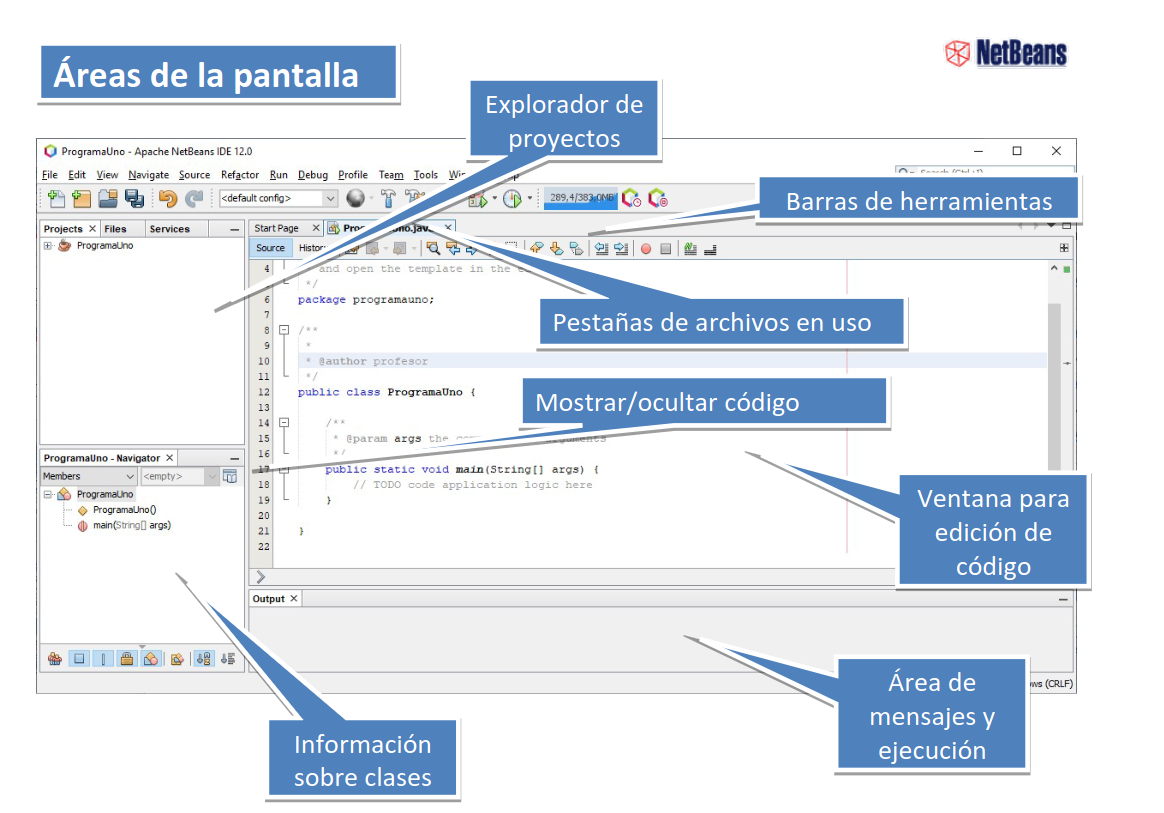
\includegraphics[scale=0.40]{netbeans-1.png}
    \caption{Ventana de proyecto de Netbeans}
\end{figure}

Cuando trabajemos con Netbeans nuestros proyectos harán usos de clases para poder desarrollar las operaciones de nuestros programas. Estas clases se agrupan en paquetes. En las siguientes figuras se muestra un esquema de como se gestiona la creación de paquetes.


% Bibliography

\newpage
\addcontentsline{toc}{chapter}{Bibliografía}
\bibliography{citas}
\bibliographystyle{unsrt}

\end{document}